% Modified 31 Oct 2005:  Conditioning fallacy alluded to.
% This chapter has been modified on 6-4-05.
% There are two \choice
\pagestyle{headings}
\chapter{Sets \& Counting} \label{chp 2}

\section{Sets and Set Notation}

Sets formalize the concept of a collection, and the language of set theory is ubiquitous in many branches of mathematics, so being familiar with the language and notation of set theory will be useful not only in this course, but also in mathematics more generally.

\begin{definition}
A \newterm{set}\index{Set} is an unordered collection of objects, called its \newterm{elements}\index{Element}, which could be anything. Typically we denote sets with capital letters, and elements of sets with lower case letters when we want to make a clear distinction.
\end{definition}

\begin{example}
Let $A = \{\heartsuit, p, 2, 3, \diamondsuit\}$. This set has five elements. Note that if $B = \{3,2,p,\heartsuit,\diamondsuit\}$, then $A = B$. Sets are equal when they have the same elements.
\end{example}

\begin{keypoint}
Sets have no notion of ordering or repetition. The sets $S =\{a,b,c\}$ and $T=\{c,b,b,a\}$ are equal. You'll never (from now on) see an element repeated in a set for this reason. \end{keypoint}

It's helpful to conceive of a set as a way of dividing the entire universe into two groups, the things that are in the set, and the things that are not. When asked whether any particular thing is in the set, there is always a definitive answer of yes or no. Two sets are equal when the answers to that question always agree.

\subsection*{Elements and Subsets}

If $a$ is an element of the set $A$, we write $a \in A$, and if not, we write $a \not\in A$. If $A = \{\heartsuit, p, 2, 3, \diamondsuit\}$ then $\heartsuit \in A$ and $2 \in A$, but $1 \not\in A$. The set $S$ satisfying $p \in S$ and $q \in S$, but $x \not\in S$ for all other $x$ can be written as $S = \{p,q\}$.

\begin{example}
Let $S = \{2,3,5,7\}$ and $T = \{5,10,15\}$. Then $15 \not\in S$, but $15 \in T$.
\end{example}

If $A$ and $B$ are sets, and every element of $A$ is also an element of $B$, we say that $A$ is a \newterm{subset}\index{Subset} of $B$, and write $A \subseteq B$. Notice that every set is a subset of itself.

\begin{example}
Let $X = \{2,3,5,7,9\}$, $Y = \{2,5,6\}$, and $Z = \{2,7,9\}$. Then $Z \subseteq X$. However, $Y \not\subseteq X$ since $6$ is an element of $Y$, but it's not an element of $X$.
\end{example}

\begin{example}
Let $P = \{a,b,c,d\}$. Then $c \in P$ and $\{c\} \subseteq P$. Note that $\{c\} \not \in P$ (there are four elements of $P$ and $\{c\}$ is not one of them) and $c \not\subseteq P$ ($c$ is not a set, so cannot be a subset of anything).
\end{example}

One set that comes up often enough that it's deserving of its own name is the set with no elements, known as the \newterm{empty set}\index{Empty Set}, and denoted $\emptyset = \{\}$. When asked whether anything is in $\emptyset$, the answer is always no. Note that $\emptyset \subseteq A$ for any set $A$, since if not, there would have to be something in $\emptyset$ which is not an element of $A$, but $\emptyset$ has no elements, so the statement $\emptyset \subseteq A$ is vacuously true.

In some contexts, we also define a \newterm{universal set}\index{Universal Set} $U$ as the set of all objects in the universe we are considering. For example, if we're in a setting where the only objects being considered are real numbers, we can let $U = \mathbb{R}$.

\begin{example}
Consider a single roll of a six-sided die. Let $U = \{1,2,3,4,5,6\}$. If we define $L$ as the set of outcomes which are less than five, then $L = \{1,2,3,4\}$, and if we define $E$ as the set of outcomes which are even, then $E = \{2,4,6\}$.
\end{example}

One useful way to describe a set is with \newterm{set comprehension}\index{Set Comprehension}. This notation builds a new set out of a known one by selecting only those elements that satisfy a given condition. The condition can be specified in algebraic notation, in written language, or a mix of the two. The point is that the condition is clear and unambiguous to the reader.

\begin{example}
Let $S = \{1,2,3,4,5\}$, and define $T = \{x \in S \, | \, x > 3\}$. Then $T = \{4,5\}$.
\end{example}

\begin{example}
The set $\{\frac{p}{q} \in \mathbb{Q} \, | \, q=2 \text{ and $p$ is positive}\}$ is the set of positive half-integers. These are the positive numbers which are either a whole number, or halfway between two whole numbers.
\end{example}

\section{Operations on Sets}

Given two sets $A, B \subseteq U$, we'll define four fundamental operations, the \newterm{union}\index{Union} $A \cup B$, the \newterm{intersection}\index{Intersection} $A \cap B$, the \newterm{complement}\index{Complement} $A^c$, and the \newterm{difference}\index{Difference} $A \setminus B$.

\begin{center}
\begin{minipage}{1.6in}
\begin{center}
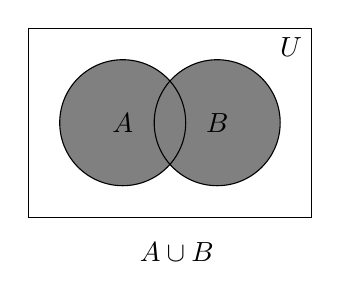
\begin{tikzpicture}[scale=0.8]
\draw (-1.5,-1.5) rectangle (3.0,1.5) node[below left]{$U$};
\draw (1.6,-1.75) node[below left]{$A \cup B$};
\begin{scope}                       % start of clip scope
\clip (0,0) circle (1cm);
\fill[gray] (0,0) circle (1cm);
\end{scope}                         % end of clip scope
\begin{scope}                       % start of clip scope
\clip (1.5,0) circle (1cm);
\fill[gray] (1.5,0) circle (1cm);
\end{scope}                         % end of clip scope
\draw (0,0) circle (1cm) node[] {$A$};
\draw (1.5,0) circle (1cm) node[] {$B$};
\end{tikzpicture}
\end{center}
\end{minipage}
\qquad\begin{minipage}{1.6in}
\begin{center}
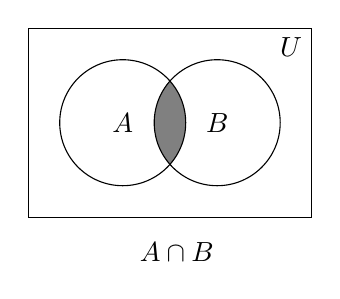
\begin{tikzpicture}[scale=0.8]
\draw (-1.5,-1.5) rectangle (3.0,1.5) node[below left]{$U$};
\draw (1.6,-1.75) node[below left]{$A \cap B$};
\begin{scope}                       % start of clip scope
\clip (0,0) circle (1cm);
\fill[white] (0,0) circle (1cm);
\end{scope}                         % end of clip scope
\begin{scope}                       % start of clip scope
\clip (1.5,0) circle (1cm);
\fill[white] (1.5,0) circle (1cm);
\end{scope}                         % end of clip scope
\begin{scope}                       % start of clip scope
\clip (0,0) circle (1cm);
\fill[gray] (1.5,0) circle (1cm);
\end{scope}                         % end of clip scope
\draw (0,0) circle (1cm) node[] {$A$};
\draw (1.5,0) circle (1cm) node[] {$B$};
\end{tikzpicture}
\end{center}
\end{minipage}
\end{center}

\begin{center}
\begin{minipage}{1.6in}
\begin{center}
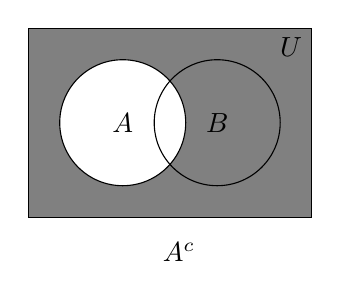
\begin{tikzpicture}[scale=0.8]
\begin{scope}                       % start of clip scope
\fill[gray] (-1.5,-1.5) rectangle (3.0,1.5);
\draw (1.3,-1.75) node[below left]{$A^c$};
\fill[white] (0,0) circle (1cm);
\end{scope}                         % end of clip scope
\draw (0,0) circle (1cm) node[] {$A$};
\draw (1.5,0) circle (1cm) node[] {$B$};
\draw (-1.5,-1.5) rectangle (3.0,1.5) node[below left]{$U$};
\end{tikzpicture}
\end{center}
\end{minipage}\qquad\begin{minipage}{1.6in}
\begin{center}
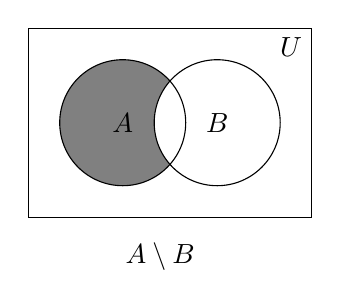
\begin{tikzpicture}[scale=0.8]
\begin{scope}                       % start of clip scope
\fill[gray] (0,0) circle (1cm);
\draw (1.3,-1.75) node[below left]{$A \setminus B$};
\fill[white] (1.5,0) circle (1cm);
\end{scope}                         % end of clip scope
\draw (0,0) circle (1cm) node[] {$A$};
\draw (1.5,0) circle (1cm) node[] {$B$};
\draw (-1.5,-1.5) rectangle (3.0,1.5) node[below left]{$U$};
\end{tikzpicture}
\end{center}
\end{minipage}
\end{center}

One can interpret $\cup$ as `or', $\cap$ as `and', and $^{c}$ as `not', but remember that $\cup$ refers to the \emx{inclusive or}, as in `to participate you must be older than 16 or have permission of a parent' (\emx{possibly both!}), not the \emx{exclusive or}, as in `the meal comes with a choice of soup or salad' (\emx{not both!}).

\begin{warning}
In colloquial language, the word `or' is ambiguous. The set $A \cup B$ is the set of all elements that are in $A$ or in $B$ or in both.
\end{warning}

The set difference $A \setminus B$ is what remains when all elements of $B$ are removed from the set $A$. Note that we can express this as $A \setminus B = A \cap B^c$ (the set of elements which are in $A$ \emx{and} \emx{not} in $B$), so the difference operation does not add any more expressive power to the language, since it can be defined in terms of the others. However, it's often a convenient shorthand.

\begin{example}
Let $U = \{p,q,r,s,t,u,v\}$, and take $A = \{p,q,r,s\}$ and $B = \{p,r,t,v\}$. Then we can compute $A \cap B = \{p,r\}$, $A^c = \{t,u,v\}$, and $(A \cup B)^c = (\{p,q,r,s,t,v\})^c = \{u\}$.
\end{example}

\begin{example}
Let $U = \{\heartsuit,\diamondsuit,\clubsuit,\spadesuit\}$, and take $S = \{\heartsuit,\diamondsuit,\clubsuit\}$ and $T = \{\heartsuit\}$. Then we can compute $S \setminus T = \{\diamondsuit,\clubsuit\}$ and $T \setminus S = \emptyset$.
\end{example}

\subsection*{The Algebra of Sets}

The set operations described above satisfy certain algebraic laws. For the most part, these laws should seem intuitively clear once you've had enough experience with the set operations, and for this reason, you should not attempt to memorize them. The exceptions, however, are the \newterm{distributive laws}\index{Distributive Laws}\ and \newterm{DeMorgan's laws}\index{DeMorgan's Laws}, which take some getting used to, and are not (at least to me and most others) immediate from the meaning of the operations.

\renewcommand{\arraystretch}{1.5}
\begin{center}
\begin{tabular}{@{} >{\bfseries}l >{\arraybackslash}m{6.5cm} @{}}

\hline

Identity & $A \cup \emptyset = A$, \quad $A \cap U = A$ \\

Domination & $A \cup U = U$, \quad $A \cap \emptyset = \emptyset$ \\

Idempotent & $A \cup A = A$, \quad $A \cap A = A$ \\

Complement & $A \cup A^c = U$, \quad $A \cap A^c = \emptyset$, \quad $(A^c)^c = A$ \\

Commutative & $A \cup B = B \cup A$, \quad $A \cap B = B \cap A$ \\

Absorption & $A \cup (A \cap B) = A$, \quad $A \cap (A \cup B) = A$ \\

Associative & $(A \cup B) \cup C = A \cup (B \cup C)$ \\ 
			& $(A \cap B) \cap C = A \cap (B \cap C)$ \\

Distributive & $A \cup (B \cap C) = (A \cup B) \cap (A \cup C)$ \\
             & $A \cap (B \cup C) = (A \cap B) \cup (A \cap C)$ \\

De Morgan's & $(A \cup B)^c = A^c \cap B^c$, \quad $(A \cap B)^c = A^c \cup B^c$ \\

\hline

\end{tabular} 
\end{center}

\begin{example}
Use laws of set algebra to simplify the expression $(A \cup (B \cap A^c)) \setminus B$.
$$\begin{aligned}
(A \cup (B \cap A^c)) \setminus B &= (A \cup (B \cap A^c)) \cap B^c \\
&= ((A \cup B) \cap (A \cup A^c)) \cap B^c \\
&= ((A \cup B) \cap U) \cap B^c \\
&= (A \cup B) \cap B^c \\
&= (A \cap B^c) \cup (B \cap B^c) \\
&= (A \cap B^c) \cup \emptyset \\
&= A \cap B^c \\
\end{aligned}$$
\end{example}

\begin{remark}
The example above might leave you with some questions. Why were the laws used in that particular order? What does it even mean for one set expression to be `simpler' than another?

Questions like these are addressed in a branch of mathematics known as Boolean algebra, which we're just scratching the surface of. Take the example as an illustration of how the laws above can be used in a productive way, and an invitation to think about some of the basic questions in Boolean algebra, the answers to which are beyond the scope of this course.
\end{remark}

\section{Inclusion-Exclusion Principle}\label{InclusionExclusionSec}

The number of elements in a set $A$ is known as its \newterm{cardinality}\index{Cardinality}, denoted $N(A)$ or $|A|$. Note that sets can have infinitely many elements, and we will write $N(A) = \infty$ when this occurs.

\begin{example}
Let $A = \{\heartsuit, \spadesuit, \diamondsuit\}$, and $B = \{\frac{1}{2}, \frac{1}{4},\frac{1}{8},\frac{1}{16}, \dots\}$. Then $N(A) = 3$ and $N(B) = \infty$.
\end{example}

There is only one set whose cardinality is zero, the empty set $\emptyset$. There are countless sets whose cardinality is infinite. The set $B$ in the example above, the natural numbers $\mathbb{N} = \{0,1,2,3,4,\dots\}$, the integers $\mathbb{Z} = \{\dots, -2, -1, 0 ,1 ,2, \dots\}$, and the real numbers $\mathbb{R}$ are examples you've encountered before.

It's important, and may come as a surprise, to know that some of these infinite sets have more elements than others. The sets $\mathbb{N}$, $\mathbb{Z}$, and $\mathbb{E} = \{2,4,6, \dots\}$ (the positive even numbers) all have the same number of elements, but the set $\mathbb{R}$ has more. The classic introduction to how this works is known as \newterm{Hilbert's Hotel}.

If a set has a larger cardinality than $\mathbb{N}$, we say it's \newterm{uncountable}. If it has a finite cardinality, or the same cardinality as $\mathbb{N}$, we say it's \newterm{countable}.

In the case where the cardinalities $N(A)$ and $N(B)$ are both finite, there is an important relationship between $N(A)$, $N(B)$, $N(A \cup B)$, and $N(A \cap B)$ that's very useful when calculating probabilities, which we'll get to in the next chapter.

\begin{theorem}
(Inclusion-Exclusion Principle) $N(A \cup B) = N(A) + N(B) - N(A \cap B)$.
\end{theorem}
\begin{proof} Consider the sum $N(A) + N(B)$. Every element in exactly one of the two sets $A$ and $B$ is counted once in this sum, but an element which is in both sets (that is, an element of $A \cap B$) is counted twice.

\begin{center}
\begin{tikzpicture}[scale=0.8]
\draw (-1.5,-1.5) rectangle (3.0,1.5) node[below left]{$U$};
\begin{scope}                       % start of clip scope
\clip (0,0) circle (1cm);
\fill[pattern=north west lines, pattern color=gray] (0,0) circle (1cm);
\end{scope}                         % end of clip scope
\begin{scope}                       % start of clip scope
\clip (1.5,0) circle (1cm);
\fill[pattern=north east lines, pattern color=gray] (1.5,0) circle (1cm);
\end{scope}                         % end of clip scope
\draw (0,0) circle (1cm) node[] {$A$};
\draw (1.5,0) circle (1cm) node[] {$B$};
\end{tikzpicture}
\end{center}

In $N(A \cup B)$, every element of $A \cup B$ (including those in $A \cap B$) is counted only once. To count the elements in $A \cap B$ twice, as above, we can sum $N(A \cup B) + N(A \cap B)$. Thus, $N(A \cup B) + N(A \cap B) = N(A) + N(B)$, and rearranging gives $N(A \cup B) = N(A) + N(B) - N(A \cap B)$.

\end{proof}

\begin{example}
How many cards in a standard deck (52 cards, 13 of each suit) are hearts or face cards?

If we let $U$ be the set of all cards in the deck, $H$ the set of all hearts, and $F$ the set of all face cards (the J, Q, and K of each suit), then $N(H \cap F) = 3$ (the J, Q, and K of hearts), and hence
$$N(H \cup F) = N(H) + N(F) - N(H \cap F) = 13 + 12 - 3 = 22.$$
\end{example}

The inclusion-exclusion principle can be extended to unions of three sets or more. In the case of three, if we write $N(A \cup B \cup C) = N(A) + N(B) + N(C)$ then we have double counted the outcomes in the lined areas in the Venn diagram below, and triple counted the outcomes in $A \cap B \cap C$ (the shaded central area).

\begin{center}
\begin{tikzpicture}[scale=0.7]
\begin{scope}                       % start of clip scope
\clip (-1,0.67) circle (1.5cm);
\fill[pattern=north west lines, pattern color=black] (1,0.67) circle (1.5cm);
\end{scope}                         % end of clip scope
\begin{scope}                       % start of clip scope
\clip (0,-1) circle (1.5cm);
\fill[pattern=north west lines, pattern color=black] (1,0.67) circle (1.5cm);
\end{scope}                         % end of clip scope
\begin{scope}                       % start of clip scope
\clip (0,-1) circle (1.5cm);
\fill[pattern=north west lines, pattern color=black] (-1,0.67) circle (1.5cm);
\end{scope}                         % end of clip scope
\begin{scope}                       % start of clip scope
\clip (-1,0.67) circle (1.5cm);
\clip (1,0.67) circle (1.5cm);
\fill[gray] (0,-1) circle (1.5cm);
\end{scope}                         % end of clip scope
\draw (-1,0.67) circle (1.5cm) node[above left] {$A$};
\draw (1,0.67) circle (1.5cm) node[above right] {$B$};
\draw (0,-1) circle (1.5cm) node[below] {$C$};
\draw (-3.0,-3.0) rectangle (3.0,3.0) node[below left]{$U$};
\end{tikzpicture}
\end{center}

To correct for double counting the lined areas, we can subtract the cardinalities of $A \cap B$, $B \cap C$, and $C \cap A$, but each of these includes $A \cap B \cap C$. Elements of this triple intersection are counted three times and subtracted out three times. Thus, we need to add them back in to count them once. All together we obtain the formula below.
$$\begin{aligned}
N(A \cup B \cup C) &= N(A) + N(B) + N(C)\\ &\  - N(A \cap B) - N(B \cap C) - N(C \cap A) \\ & \ + N(A \cap B \cap C)
\end{aligned}$$

\begin{example}
At a daycare, 24 children will eat Apples, 28 children will eat Bananas, and 30 children will eat Clementines. If 18 will eat Apples \& Bananas, 22 will eat Bananas \& Clementines, 19 will eat Apples \& Clementines, and 14 will eat all three fruits, how many children will eat at least one of the three?
$$\begin{aligned}
N(A \cup B \cup C) &= N(A) + N(B) + N(C)\\ &\  - N(A \cap B) - N(B \cap C) - N(C \cap A) \\ & \ + N(A \cap B \cap C) \\
&= 24 + 28 + 30 - 18 - 22 - 19 + 14 \\
&= 37
\end{aligned}$$
\end{example}

Notice that when we apply the inclusion-exclusion principle, we can solve for any of the terms. If we were given the cardinality of the union of all three sets, we could instead solve for the cardinality of the intersection of all three sets.

\begin{example}
At a daycare, 24 children will eat Apples, 28 children will eat Bananas, and 30 children will eat Clementines. If 18 will eat Apples \& Bananas, 22 will eat Bananas \& Clementines, 19 will eat Apples \& Clementines, and 37 will eat at least one of the three fruits, how many children will eat all three?
$$\begin{aligned}
N(A \cup B \cup C) &= N(A) + N(B) + N(C)\\ &\  - N(A \cap B) - N(B \cap C) - N(C \cap A) \\ & \ + N(A \cap B \cap C) \\
37 &= 24 + 28 + 30 - 18 - 22 - 19 + N(A \cap B \cap C) \\
14 &= N(A \cap B \cap C)
\end{aligned}$$
\end{example}

These kind problems can also be done by filling in the regions of the Venn diagram carefully with the correct counts, while being very careful to never double count. In many cases, this approach is faster and more natural then writing out the algebraic form of the law.

\begin{example}
At a daycare, 24 children will eat Apples, 28 children will eat Bananas, and 30 children will eat Clementines. If 18 will eat Apples \& Bananas, 22 will eat Bananas \& Clementines, 19 will eat Apples \& Clementines, and 14 will eat all three fruits, how many children will eat only apples, and neither of the other two fruits?

We'll start with the count in the centre, 14, and move from the inside out. 

\begin{center}
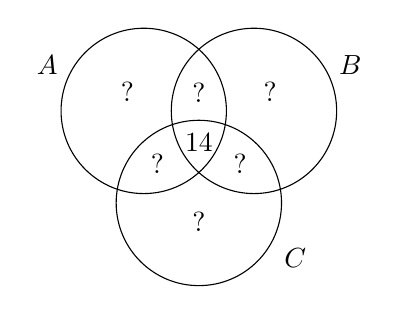
\begin{tikzpicture}[scale=0.7]
\draw (-2.75,1.5) node {$A$};
\draw (2.75,1.5) node {$B$};
\draw (1.75,-2) node {$C$};
\draw (-1,0.67) circle (1.5cm) node[above left] {$?$};
\draw (1,0.67) circle (1.5cm) node[above right] {$?$};
\draw (0,-1) circle (1.5cm) node[below] {$?$};
\draw (0,0.1) node {$14$};
\draw (0,1) node {$?$};
\draw (-0.75,-0.3) node {$?$};
\draw (0.75,-0.3) node {$?$};
\end{tikzpicture}
\end{center}

Since $N(A \cap B) = 18$, and the 14 children in the centre will all eat Apples and Bananas, the region directly above the centre has 4 children in it, that is, there are 4 children who will eat Apples and Bananas but not Clementines ($A \cap B \cap C^c$). Similarly, since $N(A \cap C) = 19$ and $N(A \cap B \cap C) = 14$, there are 5 children who will eat Apples and Clementines but not Bananas ($A \cap B^c \cap C$).

\begin{center}
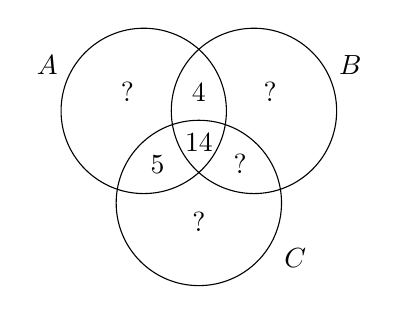
\begin{tikzpicture}[scale=0.7]
\draw (-2.75,1.5) node {$A$};
\draw (2.75,1.5) node {$B$};
\draw (1.75,-2) node {$C$};
\draw (-1,0.67) circle (1.5cm) node[above left] {$?$};
\draw (1,0.67) circle (1.5cm) node[above right] {$?$};
\draw (0,-1) circle (1.5cm) node[below] {$?$};
\draw (0,0.1) node {$14$};
\draw (0,1) node {$4$};
\draw (-0.75,-0.3) node {$5$};
\draw (0.75,-0.3) node {$?$};
\end{tikzpicture}
\end{center}

Finally, $N(A) = 24$, and three of the four regions that make up $A$ have been filled out, and total $14+4+5 = 23$ children. Thus, only a single child eats Apples and none of the other fruits ($A \cap B^c \cap C^c$). 

\begin{center}
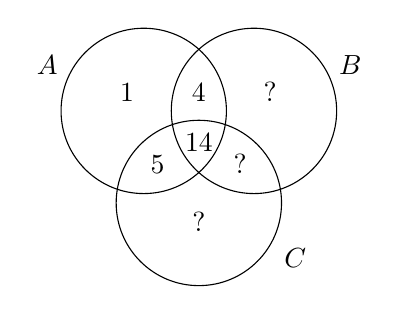
\begin{tikzpicture}[scale=0.7]
\draw (-2.75,1.5) node {$A$};
\draw (2.75,1.5) node {$B$};
\draw (1.75,-2) node {$C$};
\draw (-1,0.67) circle (1.5cm) node[above left] {$1$};
\draw (1,0.67) circle (1.5cm) node[above right] {$?$};
\draw (0,-1) circle (1.5cm) node[below] {$?$};
\draw (0,0.1) node {$14$};
\draw (0,1) node {$4$};
\draw (-0.75,-0.3) node {$5$};
\draw (0.75,-0.3) node {$?$};
\end{tikzpicture}
\end{center}

\end{example}

\begin{keypoint}
Always fill in the Venn diagram from the inside out. Even if the quantity you're solving for is in the center, call it $x$ and start filling in from the center, moving out.
\end{keypoint}

\begin{example}
In a group of 45 people, 31 of them went swimming, 26 of them went canoeing, and 7 of them did neither activity. How many did both activities?

\begin{center}
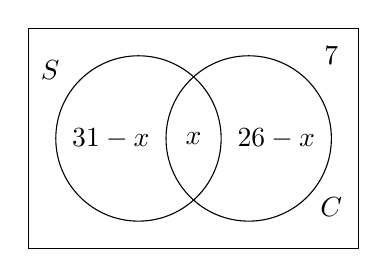
\begin{tikzpicture}[scale=0.7]
\draw (-1.6,1.25) node {$S$};
\draw (3.5,-1.25) node {$C$};
\draw (-2,-2) rectangle (4.0,2);
\draw (0,0) circle (1.5cm);
\draw (2,0) circle (1.5cm);
\draw (1,0) node[] {$x$};
\draw (3.5,1.5) node[] {$7$};
\draw (-0.5,0) node[] {$31-x$};
\draw (2.5,0) node[] {$26-x$};
\end{tikzpicture}
\end{center}

Let $x$ be the number of people that did both activities. If we label the Venn diagram as above and sum the values in all four regions, then $(31-x) + x + (26-x) + 7 = 45$. Solving yields $x = 19$.

Alternatively, we could use the algebraic form of the inclusion-exclusion principle, after noting that since 7 people did neither activity, $N((S \cup C)^c) = 7$, and hence $N(S \cup C) = 45 - 7 = 38$. Now applying the inclusion-exclusion principle,
$$\begin{aligned}
N(S \cup C) &= N(S) + N(C) - N (S \cap C) \\
38 &= 31 + 26 - N (S \cap C) \\
N (S \cap C) &= 31 + 26 - 38 \\
N (S \cap C) &= 19
\end{aligned}$$

\end{example}

\section{Counting Principles \& Factorials}

Suppose you order fries and root beer at a fast food restaurant. There are two options for the size of the fries and three options for the size of the root beer.

Since there are two options for the size of the fries, and three options for the size of the root beer, you have a total of six possible choices when you order both. These are enumerated below, the first letter in each ordered pair denoting the size of the fries (small or large), and the second letter the size of the root beer (small, medium, or large).
$$(S,s)\ \ (S,m)\ \ (S,l)\ \ (L,s)\ \ (L,m)\ \ (L,l)$$
These are exactly the elements of the cartesian product $F \times R$, where $F = \{S,L\}$ and $R = \{s,m,l\}$. 

If it turns out that, unfortunately, there's only enough change in your pocket to pay for a single item (which could be any size), then you only have five choices. Either you only order fries, and choose an element from $F$, or only order root beer, and choose an element from $R$. This is equivalent to choosing an element of $F \cup R = \{S,L,s,m,l\}$.

To summarize, the number of ways to choose an element from $F$ \emx{and} an element from $R$ is $|F| \cdot |R|$, while the number of ways to choose an element from $F$ \emx{or} an element from $R$ is $|F|+|R|$. This idea generalizes considerably, and forms the foundational principle that will allow us to solve many problems.

\begin{proposition}(Fundamental Counting Principle) \label{FundamentalCountingPrinciple}\index{Fundamental Counting Principle} In a sequence of $k$ choices, if the first choice can be made in $n_1$ ways, the second choice can be made in $n_2$ ways, and so on, the number of ways of making all choices is the product $n_1 n_2 \,\cdots\, n_k$, while the number of ways of selecting one of the choices to make and making only that choice is the sum $n_1 + n_2 + \,\cdots\, + n_k$.
\end{proposition}

\begin{example}
How many ways are there to select three students to be class representatives in three different classes, one with twenty students and two with thirty?

There are three choices to be made, choosing a representative for each of the three classes, and since we must make all three choices, the number of ways this can be done is $20 \cdot 30 \cdot 30 = 18\,000$.
\end{example}

\begin{example}
How many four symbol sequences can be made with the symbols in $S = \{\heartsuit, \diamondsuit, \clubsuit, \spadesuit\}$?

We can imagine filling in four blank spaces with symbols, and write in each blank space the number of choices we have for the symbol that gets placed there. If we allow the same letter to be used many times, then the number of sequences is $\underline{4} \cdot \underline{4} \cdot \underline{4} \cdot \underline{4} = 256$.

On the other hand, if each space must be filled with a distinct symbol, then initially there are four choices for the first symbol, but after making that choice, there are three remaining for the second symbol, and so on. In total then, the number of sequences with distinct symbols is $\underline{4} \cdot \underline{3} \cdot \underline{2} \cdot \underline{1} = 24$. 
\end{example}

This second result is the number of ways of arranging four different symbols in a line, and counting arrangements is something we'll do frequently, so it's convenient to have a shorthand for this kind of descending product of consecutive integers.

\begin{definition}\index{Factorial}
Given $n \in \mathbb{N}$, the \newterm{factorial} of $n$, denoted $n!$, is the number of ways of arranging $n$ distinct objects in a line, and is defined by
$$n! = n \cdot (n-1) \cdot (n-2) \cdot \, \cdots \, \cdot 2 \cdot 1$$
\end{definition}

\begin{note} Though the usual interpretation of the factorial in terms of counting arrangements no longer applies, we define $0!=1$ for convenience. This makes many formulas involving factorials (like the Taylor series formula) much easier to write.
\end{note}

Factorials have some very nice algebraic properties that make them easy to work with, in particular, ratios of factorials can be simplified easily.
\eqnsgap{\frac{8!}{6!} = \frac{8 \cdot 7 \cdot 6 \cdot 5 \cdot 4 \cdot 3 \cdot 2 \cdot 1}{6 \cdot 5 \cdot 4 \cdot 3 \cdot 2 \cdot 1}= \frac{8 \cdot 7 \cdot \cancel{6} \cdot \cancel{5} \cdot \cancel{4} \cdot \cancel{3} \cdot \cancel{2} \cdot \cancel{1}}{\cancel{6} \cdot \cancel{5} \cdot \cancel{4} \cdot \cancel{3} \cdot \cancel{2} \cdot \cancel{1}} = 56}
\par

%Factiorial algebra examples

\section{Permutations \& Combinations}

\subsection*{Permutations}\label{PermutationsSec}

\begin{example}
How many ways are there to choose three students from a class of twenty and arrange them in a line?

We can use the same approach as in the last example. We're filling in three blanks, we have twenty options to choose from, and repeats are not permitted. Thus, there are $\underline{20} \cdot \underline{19} \cdot \underline{18} = 6\,840$ ways to do it. 

\noindent The notation $^{20}P_3$ is used to refer to the number of ways of selecting $3$ objects from a set of $20$ distinct options and ordering them. Thus, we have $^{20}P_3 = 6\,840$.
\end{example}

\begin{definition}\label{permutationdefinition}\index{Permutations}
If an ordered list of $r$ distinct objects is selected from a set of $n$ objects, the result is called an $r$-\newterm{permutation}. The number of $r$-permutations of $n$ objects, denoted by $^{n}P_r$, is given by
$$^nP_r = n \cdot (n-1) \cdot \, \cdots \, \cdot (n-r+1) = \frac{n!}{(n-r)!}$$
\end{definition}

\begin{remark}
We can write the formula for permutations conveniently as above, but it's usually more helpful in problems to think about the fundamental counting principle directly, and to interpret the formula for permutations as a truncated factorial (a factorial with the end cut off).
\end{remark}

\begin{example}
How many ways are there to create a sequence of five letters with no repetitions using any of the 26 lower case letters of the alphabet?

Taking $5$ letters from a set of $26$ and arranging them, the number of options is
$$^{26}P_5 = \frac{26!}{(26-5)!} = \frac{26!}{21!} = 26 \cdot 25 \cdot 24 \cdot 23 \cdot 22 = 7\,893\,600$$
\end{example}

%More examples

\subsection*{Permutations with Identical Objects}

What if some objects are indistinguishable? If this is the case, there are fewer possibilities. For example, how many arrangements of the letters in the string $AAAB$ are there? 

Notice that we just have to decide which of the four possible positions we'll place the $B$ into. Once that's done, then $A$'s go everywhere else, so there are only four distinct arrangements.

Now suppose that we number the three $A$s. How many rearrangements of the string $A_1A_2A_3B$ are there? Since the four letters are now distinguishable, there are $4! = 24$. Let's write these out, grouping together in columns all strings that will be identical after the labels on the $A$'s are removed.
\begin{center}
\begin{tabular}{cccc}
$A_1A_2A_3B$ & $A_1A_2BA_3$ & $A_1BA_2A_3$ & $BA_1A_2A_3$ \\
$A_1A_3A_2B$ & $A_1A_3BA_2$ & $A_1BA_3A_2$ & $BA_1A_3A_2$ \\
$A_2A_1A_3B$ & $A_2A_1BA_3$ & $A_2BA_1A_3$ & $BA_2A_1A_3$ \\
$A_2A_3A_1B$ & $A_2A_3BA_1$ & $A_2BA_3A_1$ & $BA_2A_3A_1$ \\
$A_3A_1A_2B$ & $A_3A_1BA_2$ & $A_3BA_1A_2$ & $BA_3A_1A_2$ \\
$A_3A_2A_1B$ & $A_3A_2B_1A$ & $A_3BA_2A_1$ & $BA_3A_2A_1$ \\
\end{tabular}
\end{center}
Notice that rearranging the labels will result in a string which is identical once the labels are removed. This means if we list all possible arrangements of the labeled strings, each possible unlabeled string will appear $3!$ times, since there are $3!$ ways of arranging the labels. Alternatively, think about how there are 3! ways to \emx{apply the labels} to the three $A$'s, and each of the 24 labeled strings can be obtained by first selecting an unlabeled string (i.e. a column) then applying the labels.

The upshot is that \emx{we can count the number of unlabeled strings by dividing the number of labeled strings by the number of ways of rearranging the labels}, in this case, $4! / 3! = 4$. The same principle applies if there are many different kinds of indistinguishable objects, and the general result can be summarized in the formula below.

\begin{proposition}\index{Mississippi Formula} (Mississippi Formula) The number of ways of rearranging $n$ objects, with indistinguishable groups of sizes $k_1, k_2, \dots\, ,k_m$, is given by
$$\frac{n!}{k_{1}! \cdot k_{2}! \cdot \, \cdots \, \cdot k_{m}!}$$
\end{proposition}

\begin{example}
How many arrangements of the letters in MISSISSIPPI are there?
\par
\noindent There are eleven letters in total, with identical groups of size 4 (the I's), 4 (the S's), and 2 (the P's). Therefore, the number of arrangements is
\eqnsbiggap{\frac{11!}{4! \cdot 4! \cdot 2!} = \frac{11 \cdot 10 \cdot 9 \cdot {8} \cdot 7 \cdot {6} \cdot 5 \cdot {4} \cdot {3} \cdot {2} \cdot 1}{{4} \cdot {3} \cdot {2} \cdot 1 \cdot {4} \cdot {3} \cdot {2} \cdot 1 \cdot {2} \cdot 1} = 11 \cdot 10 \cdot 9 \cdot 7 \cdot 5 = 34\,650.}
\end{example}

\begin{example}
An urn contains four green and five red marbles, which are removed one at a time. How many different sequences of red and green marbles can result from this process?
\par
\noindent In this case, we are rearranging nine objects, four $G$'s and five $R$'s. Each arrangement, read left to right, corresponds to a sequence of marbles that could appear. There are identical groups of size 4 (the green marbles), and 5 (the red marbles). Therefore, the number of arrangements is
\eqnsbiggap{\frac{9!}{4! \cdot 5!} = \frac{9 \cdot {8} \cdot 7 \cdot {6} \cdot 5 \cdot {4} \cdot {3} \cdot {2} \cdot 1}{{4} \cdot {3} \cdot {2} \cdot 1 \cdot {5} \cdot {4} \cdot {3} \cdot {2} \cdot 1} = 9 \cdot 2 \cdot 7 = 126.}
\end{example}

\subsection*{Combinations}

Suppose now we're interested in the number of ways that a subset of $r$ objects can be selected from a larger set of $n$ distinct objects. We're only concerned with which objects are selected not with their order, so if the same objects appear, but in a different order, we consider this to be the same outcome.

Consider how many ways there are to selecta group three children from a family with five. To do this, we can imagine lining up the children any fixed order, let's say by age. We can now specify which children are chosen using a string such as $YYNYN$, which would indicate we chose the first two children in the line as well as the fourth. In fact, every distinct five letter string made up of $Y$s and $N$s which has exactly three $Y$s will represent a different choice of three children, and every choice of three children determines such a string.

Now we can use the Mississippi formula to count the number of different choices by counting strings. Each string is a rearrangement of five objects with identical groups of sizes three and two, hence there are $\frac{5!}{3!2!} = 5 \cdot 2 = 10$ possibilities.

The general principle is that once the elements of a set have been lined up in some arbitrary order, each subset is given by an \emph{ordered} list of $Y$'s and $N$'s, where $Y$ denotes membership in the subset, and $N$ denotes non-membership. We can count the number of these ordered lists of $Y$'s and $N$'s using the Mississippi formula.

\begin{definition}\index{Combinations}\label{combinationdefinition}
If a subset of $r$ objects is selected from a set of $n$ objects, the result is called an $r$-combination. The number of $r$-\newterm{combinations}, denoted $^nC_r$, or more commonly $\binom{n}{r}$, is given by
$$^nC_r = \binom{n}{r} = \frac{n!}{r!(n-r)!}$$
\end{definition}

\begin{warning}
Note carefully the distinction between $^nP_r$ and $^nC_r$. The former counts the number of ways of selecting $r$ objects \emx{and arranging them}, while the latter is the number of selections possible when \emx{any rearrangement is regarded as the same outcome}.
\end{warning}

\begin{example}
In Lotto 6/49, if you purchase a ticket you choose 6 distinct numbers between 1 and 49. The ticket wins if its numbers match 6 distinct numbers between 1 and 49 which are randomly drawn, regardless of the order they are drawn in. How many different tickets would you need to buy to guarantee a win?

Since the order of the numbers on the ticket is irrelevant, the number of different tickets available is $\binom{49}{6} = \frac{49!}{6!43!} = 13\,983\,816$, so this is the minimum number you would need to purchase to be guaranteed one will win.
\end{example}

\begin{example}
How many ways are there to choose a president, a treasurer, and an organizing committee of three from a group of 25 people? Assume no person can hold more than one position.

There are 25 choices for president, then 24 for treasurer, then $\binom{23}{3}$ for the organizing committee. Note that when choosing the organizing committee, the order in which members are chosen is irrelevant. The committee consisting of Alice, Bob, and Chelsea and the committee consisting of Chelsea, Alice, and Bob are the same. We must make all three choices, so by the fundamental counting principle the number of possibilities is
$$25 \cdot 24 \cdot \binom{23}{3} = 1\,062\,600.$$

Notice that we could just as well have proceeded in the opposite order, that is, first chosen the organizing committee, then the treasurer, then the president, and still obtained
$$\binom{25}{3} \cdot 22 \cdot 21 = 1\,062\,600.$$
\end{example}

\begin{example}How many ways are there to divide a group of eight people into a team of three and a team of five?

To create a team of three and a team of five, we choose three individuals for the team of three, then the five remaining make up the team of five.
$$\binom{8}{3}\binom{5}{5} = 56$$
\end{example}

\begin{example}
How many ways are there to divide a group of eight people into two teams of four?

To create two teams of four, we choose four for the first team, and those that remain make up another team of four. We have to be very careful though. In the example above the two teams were distinguishable (one has more people than the other), but here they are not. 

If we select A, B, C, and D for the first team and E, F, G, and H for the second, this results in the same outcome as selecting E, F, G, and H for the first team and A, B, C, and D for the second. Because the teams are indistinguishable, every outcome has been double counted! Thus, we need to divide out by the number of rearrangements of the teams.
$$\frac{\binom{8}{4}\binom{4}{4}}{2!} = 35$$

Notice that if the two teams were distinguishable, for example, if there were a red team and blue team with four people on each, there would be $\binom{8}{4}\binom{4}{4} = 70$ ways.

\begin{remark}
As the last example shows, it's very easy to end up inadvertently double counting, even for those with lots of experience with these kinds of problems. Solving such a problem amounts to coming up with a sequence of choices which can be made to produce each possible outcome. You need to convince yourself that your sequence of choices can not only produce every possible outcome, but produce it in a unique way (making any of the choices differently results in a different outcome).
\end{remark}
\end{example}



